\documentclass[12pt,a4paper,openany]{book}

% ─── Packages ───────────────────────────────────────────────────────────────
\usepackage[T1]{fontenc}
\usepackage[utf8]{inputenc}
\usepackage{lmodern}
\usepackage[a4paper, top=2.5cm, bottom=2.5cm, left=3cm, right=2.5cm]{geometry}
\usepackage{graphicx}
\usepackage{xcolor}
\usepackage{titlesec}
\usepackage{titletoc}
\usepackage{tocloft}
\usepackage{fancyhdr}
\usepackage{hyperref}
\usepackage{enumitem}
\usepackage{booktabs}
\usepackage{array}
\usepackage{tabularx}
\usepackage{mdframed}
\usepackage{fontawesome5}
\usepackage{tikz}
\usepackage{amsmath}
\usepackage{amssymb}
\usepackage{microtype}
\usepackage{setspace}
\usepackage{etoolbox}
\usepackage{parskip}
\usepackage{float}
\usepackage{caption}
\usepackage{subcaption}
\usepackage{multirow}
\usepackage{longtable}
\usepackage{colortbl}
\usepackage{tcolorbox}
\tcbuselibrary{skins,breakable,theorems}

% ─── Colour Palette ──────────────────────────────────────────────────────────
\definecolor{primaryblue}{HTML}{1A3A5C}
\definecolor{accentteal}{HTML}{0D7C8F}
\definecolor{lightgray}{HTML}{F5F7FA}
\definecolor{warningyellow}{HTML}{FFF3CD}
\definecolor{warningborder}{HTML}{FBBF24}
\definecolor{successgreen}{HTML}{D1FAE5}
\definecolor{successborder}{HTML}{10B981}
\definecolor{infoblue}{HTML}{DBEAFE}
\definecolor{infoborder}{HTML}{3B82F6}
\definecolor{dangered}{HTML}{FEE2E2}
\definecolor{dangerborder}{HTML}{EF4444}
\definecolor{sectiongray}{HTML}{6B7280}
\definecolor{coverbg}{HTML}{1E3A5F}

% ─── Hyperref Setup ──────────────────────────────────────────────────────────
\hypersetup{
  colorlinks=true,
  linkcolor=primaryblue,
  urlcolor=accentteal,
  citecolor=accentteal,
  pdftitle={AmarVote -- Complete System Guide},
  pdfauthor={AmarVote},
  pdfsubject={Voting Platform User Guide},
}

% ─── Custom Boxes ────────────────────────────────────────────────────────────
\tcbset{
  notebox/.style={
    enhanced, breakable,
    colback=infoblue, colframe=infoborder,
    fonttitle=\bfseries\color{primaryblue},
    title={\faInfoCircle\quad Note},
    left=6pt, right=6pt, top=4pt, bottom=4pt,
    arc=4pt
  },
  warnbox/.style={
    enhanced, breakable,
    colback=warningyellow, colframe=warningborder,
    fonttitle=\bfseries\color{orange!80!black},
    title={\faExclamationTriangle\quad Important},
    left=6pt, right=6pt, top=4pt, bottom=4pt,
    arc=4pt
  },
  tipbox/.style={
    enhanced, breakable,
    colback=successgreen, colframe=successborder,
    fonttitle=\bfseries\color{green!50!black},
    title={\faLightbulb\quad Tip},
    left=6pt, right=6pt, top=4pt, bottom=4pt,
    arc=4pt
  },
  dangerbox/.style={
    enhanced, breakable,
    colback=dangered, colframe=dangerborder,
    fonttitle=\bfseries\color{red!70!black},
    title={\faTimesCircle\quad Warning},
    left=6pt, right=6pt, top=4pt, bottom=4pt,
    arc=4pt
  },
  stepbox/.style={
    enhanced, breakable,
    colback=lightgray, colframe=primaryblue,
    fonttitle=\bfseries\color{white},
    attach boxed title to top left={xshift=10pt, yshift=-\tcboxedtitleheight/2},
    boxed title style={colback=primaryblue, arc=3pt},
    left=6pt, right=6pt, top=12pt, bottom=4pt,
    arc=4pt
  }
}

% ─── Section Formatting ──────────────────────────────────────────────────────
\titleformat{\chapter}[display]
  {\normalfont\huge\bfseries\color{primaryblue}}
  {\chaptertitlename\ \thechapter}{12pt}{\Huge}
\titlespacing{\chapter}{0pt}{-10pt}{20pt}

\titleformat{\section}
  {\normalfont\Large\bfseries\color{primaryblue}}
  {\thesection}{1em}{}
\titleformat{\subsection}
  {\normalfont\large\bfseries\color{accentteal}}
  {\thesubsection}{1em}{}
\titleformat{\subsubsection}
  {\normalfont\normalsize\bfseries\color{sectiongray}}
  {\thesubsubsection}{1em}{}

% ─── Header / Footer ─────────────────────────────────────────────────────────
\pagestyle{fancy}
\fancyhf{}
\fancyhead[LE,RO]{\small\thepage}
\fancyhead[LO]{\small\nouppercase{\rightmark}}
\fancyhead[RE]{\small\nouppercase{\leftmark}}
\fancyfoot[C]{\small\color{sectiongray}AmarVote --- Complete System Guide}
\renewcommand{\headrulewidth}{0.4pt}

% ─── Step Numbering Environment ──────────────────────────────────────────────
\newcounter{stepcount}[chapter]
\newcommand{\step}[1]{%
  \stepcounter{stepcount}%
  \begin{tcolorbox}[stepbox, title={Step \thestepcount: #1}]%
}

% ─── Custom Commands ─────────────────────────────────────────────────────────
\newcommand{\uibutton}[1]{\colorbox{primaryblue}{\textcolor{white}{\small\textbf{#1}}}}
\newcommand{\uifield}[1]{\texttt{\color{accentteal}#1}}
\newcommand{\uimenu}[1]{\textbf{\color{primaryblue}#1}}
\newcommand{\placeholder}[1]{\textit{\color{sectiongray}[#1]}}
\newcommand{\role}[1]{\textbf{\textsc{#1}}}

% ─── Figure Helper ───────────────────────────────────────────────────────────
% Usage: \screenfig[width fraction]{filename}{caption}
\newcommand{\screenfig}[3][0.92]{%
  \begin{figure}[H]
    \centering
    \includegraphics[width=#1\linewidth]{figures/#2}
    \caption{#3}
    \label{fig:#2}
  \end{figure}%
}
% Narrow figure helper (0.60 width) for CSV/file format screenshots
\newcommand{\screenfignarrow}[2]{%
  \begin{figure}[H]
    \centering
    \includegraphics[width=0.60\linewidth]{figures/#1}
    \caption{#2}
    \label{fig:narrow-#1}
  \end{figure}%
}

% ─── List Styling ────────────────────────────────────────────────────────────
\setlist[itemize,1]{label=\textcolor{accentteal}{\faChevronRight}, leftmargin=1.5em}
\setlist[itemize,2]{label=\textcolor{sectiongray}{\faCircle[regular]}, leftmargin=2em}
\setlist[enumerate,1]{label=\textcolor{primaryblue}{\textbf{\arabic*.}}, leftmargin=2em}

\setstretch{1.15}

% ════════════════════════════════════════════════════════════════════════════
\begin{document}

% ─── COVER PAGE ──────────────────────────────────────────────────────────────
\begin{titlepage}
	\pagecolor{coverbg}
	\color{white}
	\centering
	\vspace*{2cm}

	{\fontsize{60}{65}\selectfont\bfseries AmarVote}

	\vspace{0.5cm}
	{\Large\color{accentteal} Secure Cryptographic Voting Platform}

	\vspace{1.5cm}
	\hrule width 12cm height 0.5pt
	\vspace{0.4cm}
	{\LARGE\bfseries Complete System Guide}
	\vspace{0.4cm}
	\hrule width 12cm height 0.5pt

	\vspace{2cm}

	\begin{tcolorbox}[
			enhanced, width=10cm,
			colback=primaryblue!80!black, colframe=accentteal,
			arc=6pt, boxrule=1.5pt,
			left=12pt, right=12pt, top=10pt, bottom=10pt
		]
		\centering\color{white}
		\textbf{This guide covers the full end-to-end workflow of AmarVote:}\\[6pt]
		\textcolor{accentteal}{\faUser} \, Platform Setup \& Authentication\\[4pt]
		\textcolor{accentteal}{\faCog} \, Election Creation \& Configuration\\[4pt]
		\textcolor{accentteal}{\faKey} \, Guardian Key Ceremony\\[4pt]
		\textcolor{accentteal}{\faVoteYea} \, Encrypted Voting \& Benaloh Challenge\\[4pt]
		\textcolor{accentteal}{\faCalculator} \, Tallying \& Cryptographic Decryption\\[4pt]
		\textcolor{accentteal}{\faCheckDouble} \, Independent Ballot Verification
	\end{tcolorbox}

	\vfill

	\begin{tabular}{cc}
		\textcolor{accentteal}{\faLock} \, ElectionGuard Powered &
		\textcolor{accentteal}{\faLock} \, End-to-End Verifiable
	\end{tabular}

	\vspace{1cm}
	{\small Version 1.0 \quad|\quad \today}
\end{titlepage}
\nopagecolor
\color{black}

% ─── FRONT MATTER ────────────────────────────────────────────────────────────
\frontmatter
\tableofcontents

\chapter*{About This Guide}
\addcontentsline{toc}{chapter}{About This Guide}

This document is the authoritative, comprehensive reference for the \textbf{AmarVote} platform. It is written for a general audience --- no prior knowledge of cryptography, election administration, or software engineering is required.

AmarVote is built on the \textbf{ElectionGuard} specification developed by Microsoft, which guarantees \emph{end-to-end verifiability}: every voter can independently confirm that their ballot was cast as intended, recorded as cast, and counted as recorded --- without ever exposing how they voted.

\vspace{0.5cm}
\begin{tcolorbox}[notebox]
	This guide deliberately mirrors the actual workflow of the application in the exact order you would encounter it. Read sequentially for first-time use, or jump to a specific chapter if you need a quick reference.
\end{tcolorbox}

\vspace{0.5cm}

\section*{Roles at a Glance}

\begin{center}
	\begin{tabularx}{0.95\textwidth}{>{\bfseries}l X}
		\toprule
		\rowcolor{primaryblue}\color{white}Role & \color{white}Responsibilities                                                                                \\
		\midrule
		\rowcolor{lightgray}Owner               & Full platform control: manages the authorised-user list, assigns roles, and sets global permissions.         \\
		Admin                                   & Creates and administers elections, configures election parameters, and oversees the tally phase.             \\
		\rowcolor{lightgray}Guardian            & Participates in the cryptographic key ceremony; holds a share of the decryption key needed to tally results. \\
		Voter                                   & Registers, receives election access, casts an encrypted ballot, and independently verifies the result.       \\
		\bottomrule
	\end{tabularx}
\end{center}

\vspace{0.5cm}
\begin{tcolorbox}[notebox]
	\textbf{Permission hierarchy:} Owner $>$ Admin $>$ User (voter). The Owner can elevate or restrict any account. All roles require a registered account.
\end{tcolorbox}

% ════════════════════════════════════════════════════════════════════════════
\mainmatter

% ════════════════════════════════════════════════════════════════════════════
\part{Platform Foundation}

% ────────────────────────────────────────────────────────────────────────────
\chapter{Access Control \& Authorisation System}
\label{ch:access}

AmarVote is a closed platform --- not just anyone can register. Before a user can even create an account, their email address must appear on the \textbf{Authorised User List} managed by the Owner. This design ensures that elections are only accessible by vetted participants.

\section{The Authorised User List}

The Owner maintains a registry of permitted email addresses. Each entry in the list specifies:

\begin{itemize}
	\item The user's \uifield{email address}
	\item The \uifield{assigned role} (Owner, Admin, or User)
\end{itemize}

\subsection{Adding Individual Users}

\begin{enumerate}
	\item Log in to AmarVote with an Owner account.
	\item Open the navigation menu by clicking the menu icon at the top of the sidebar.

	      \screenfig{openMenu.png}{Opening the navigation menu}

	\item Navigate to \uimenu{Authenticated Users} in the sidebar.

	      \screenfig{menuSelectAuthenticatedUsers.png}{Selecting \textit{Authenticated Users} from the navigation menu}

	\item Click \uibutton{Add User}.
	\item Enter the email address in the \uifield{Email} field.
	\item Select the appropriate role from the \uifield{Role} dropdown.
	\item Click \uibutton{Save}.
\end{enumerate}

\screenfig{authenticateOneUser.png}{Adding an individual user to the Authorised User List}

\begin{tcolorbox}[tipbox]
	If you are adding a small number of users (fewer than 10), the individual entry method is faster. For larger groups, use CSV bulk upload.
\end{tcolorbox}

\subsection{Bulk Upload via CSV}

For adding many users at once:

\begin{enumerate}
	\item Prepare a \texttt{.csv} file with one column, emails\\

	      \screenfignarrow{guardiansCSVFile.png}{Example CSV format for bulk user upload}

	\item Navigate to \uimenu{Authenticated Users} $\to$ \uibutton{Import CSV}.
	\item Click \uibutton{Choose File} and select your prepared CSV.
\end{enumerate}

\screenfig{authenticateUsersWithCSVFileUpload.png}{Bulk importing users via CSV upload}

\begin{tcolorbox}[warnbox]
	Duplicate email entries in the CSV will be ignored. If an email already exists in the system, it will be ignored, not duplicated.
\end{tcolorbox}

\section{Role Capabilities Summary}

\begin{center}
	\begin{tabularx}{0.95\textwidth}{>{\bfseries}l XXXX}
		\toprule
		\rowcolor{primaryblue}\color{white}Capability           & \color{white}Owner                  & \color{white}Admin                  & \color{white}User                   \\
		\midrule
		\rowcolor{lightgray}Manage authorised-user list         & \textcolor{successborder}{\faCheck} & \textcolor{dangerborder}{\faTimes}  & \textcolor{dangerborder}{\faTimes}  \\
		Assign roles                                            & \textcolor{successborder}{\faCheck} & \textcolor{dangerborder}{\faTimes}  & \textcolor{dangerborder}{\faTimes}  \\
		\rowcolor{lightgray}Create elections (default)          & \textcolor{successborder}{\faCheck} & \textcolor{successborder}{\faCheck} & \textcolor{dangerborder}{\faTimes}  \\
		Create elections (if granted)                           & \textcolor{successborder}{\faCheck} & \textcolor{successborder}{\faCheck} & \textcolor{successborder}{\faCheck} \\
		\rowcolor{lightgray}Vote in elections                   & \textcolor{successborder}{\faCheck} & \textcolor{successborder}{\faCheck} & \textcolor{successborder}{\faCheck} \\
		View public elections                                   & \textcolor{successborder}{\faCheck} & \textcolor{successborder}{\faCheck} & \textcolor{successborder}{\faCheck} \\
		\rowcolor{lightgray}View private elections (if invited) & \textcolor{successborder}{\faCheck} & \textcolor{successborder}{\faCheck} & \textcolor{successborder}{\faCheck} \\
		\bottomrule
	\end{tabularx}
\end{center}

\begin{tcolorbox}[notebox]
	\textbf{Election creation setting:} The Owner can enable a global setting allowing \emph{all} users (not just admins) to create elections. When this setting is active, both Admins and regular Users will see the \uimenu{Create Election} button in their menu.
\end{tcolorbox}

% ────────────────────────────────────────────────────────────────────────────
\chapter{Account Registration}
\label{ch:registration}

Before using any feature of AmarVote, every participant --- voter, guardian, or admin --- must create a personal account. The registration process involves email verification and optional two-factor authentication setup.

\section{Prerequisites}

\begin{tcolorbox}[warnbox]
	You can only register if your email address has been added to the Authorised User List by an Owner. If you attempt to register with an unlisted email, the system will reject your request.
\end{tcolorbox}

\section{Step-by-Step Registration}

\subsection{Step 1 --- Navigate to Registration}

\begin{enumerate}
	\item Open your web browser and go to the AmarVote application URL.
	\item On the landing page, click \uibutton{Register} or navigate to \texttt{/register}.
\end{enumerate}

\subsection{Step 2 --- Submit Your Email Address}

\begin{enumerate}
	\item Enter your \uifield{Email Address} in the provided field. This must exactly match the email your Owner added to the authorised list.
	\item Click \uibutton{Send Verification Code}.
	\item The system will send a \textbf{One-Time Password (OTP)} to your email inbox.
\end{enumerate}

\begin{tcolorbox}[tipbox]
	Check your spam or junk folder if you do not receive the email within two minutes. The OTP is typically valid for \textbf{10 minutes}.
\end{tcolorbox}

\subsection{Step 3 --- Verify Your Email}

\begin{enumerate}
	\item Open the email from AmarVote.
	\item Copy the 6-digit verification code.
	\item Return to the registration page and enter the code in the \uifield{Verification Code} field.
	\item Click \uibutton{Verify Email}.
	\item If successful, you will be advanced to the password setup step.
\end{enumerate}

\subsection{Step 4 --- Set Your Password}

\begin{enumerate}
	\item Enter a strong password in the \uifield{Password} field. Recommended: at least 12 characters, including uppercase letters, numbers, and symbols.
	\item Re-enter the same password in the \uifield{Confirm Password} field.
	\item Click \uibutton{Create Account}.
\end{enumerate}

\begin{tcolorbox}[dangerbox]
	\textbf{Never share your password.} AmarVote staff will never ask for your password. Store it in a secure password manager.
\end{tcolorbox}

\section{Two-Factor Authentication (2FA) --- Optional but Recommended}

After your account is created, you can enable Two-Factor Authentication using \textbf{Google Authenticator} (or any TOTP-compatible app such as Authy or Microsoft Authenticator).

\subsection{Enabling 2FA}

\begin{enumerate}
	\item Log in to your new account.
	\item Click your profile avatar in the top-right corner.

	      \screenfig{goToProfileMenu.png}{Accessing the profile menu from the top-right corner}

	\item Click \uibutton{Enable Two-Factor Authentication}.
	\item A QR code will be displayed on screen.
	\item Open the Google/Microsoft Authenticator app on your smartphone.
	\item Tap the \textbf{+} button and select \uimenu{Scan a QR code}.
	\item Point your camera at the QR code on screen.
	\item Google Authenticator will display a 6-digit rotating code. Enter this code in the \uifield{Verification Code} field on AmarVote.
	\item Successful input will activate 2FA.
\end{enumerate}

\begin{tcolorbox}[warnbox]
	\textbf{Be Careful With Your 2FA!} If you lose access to your authenticator app you may be permanently locked out of your account.
\end{tcolorbox}

% ────────────────────────────────────────────────────────────────────────────
\chapter{Logging In}
\label{ch:login}

\section{Standard Login}

\begin{enumerate}
	\item Navigate to the AmarVote application and click \uibutton{Login} or go to \texttt{/login}.
	\item Enter your registered \uifield{Email Address}.
	\item Enter your \uifield{Password}.
	\item Click \uibutton{Sign In}.
\end{enumerate}

\section{Login with Two-Factor Authentication}

If you have 2FA enabled:

\begin{enumerate}
	\item Complete the email and password fields as above.
	\item Click \uibutton{Sign In}.
	\item A prompt will appear asking for your \uifield{Authenticator Code}.
	\item Open the Google Authenticator app and copy the current 6-digit code for AmarVote.
	\item Enter the code and click \uibutton{Verify}.
\end{enumerate}

\begin{tcolorbox}[notebox]
	The TOTP code rotates every 30 seconds. If the code expires while you are typing, wait for the next code to appear and use that one.
\end{tcolorbox}

\section{Forgot Password}

\begin{enumerate}
	\item On the login page, click \uimenu{Forgot Password?}.
	\item Enter your registered email address and click \uibutton{Send Reset Link}.
	\item Check your email for a password reset verification code (valid for some minutes).
	\item Verify the code and set a new password.
\end{enumerate}

% ════════════════════════════════════════════════════════════════════════════
\part{Election Administration}

% ────────────────────────────────────────────────────────────────────────────
\chapter{Creating an Election}
\label{ch:create-election}

This chapter is intended for Admins (and Users with election-creation permission). It walks through every option available when setting up a new election.

\begin{tcolorbox}[warnbox]
	The \uimenu{Create Election} button will only appear in your navigation menu if you have been granted election-creation permission. If you cannot see it, contact your Owner.
\end{tcolorbox}

\section{Accessing the Election Creation Form}

\begin{enumerate}
	\item Log in to AmarVote.
	\item Open the navigation menu by clicking the menu icon at the top of the sidebar.

	      \screenfig{openMenu.png}{Opening the navigation menu to access election management options}

	\item In the left navigation sidebar, click \uimenu{Create Election}.

	      \screenfig{menuSelectCreateElection.png}{Selecting \textit{Create Election} from the navigation menu}

	\item The \textbf{New Election} form will open.
\end{enumerate}

\section{Basic Election Information}

\subsection{Election Name \& Description}

\begin{itemize}
	\item \uifield{Election Name}: A short, descriptive title (e.g., ``Student Council Election 2025'').
	\item \uifield{Description}: A longer explanation of the election's purpose, visible to voters.
\end{itemize}

\subsection{Visibility: Public vs.\ Private}

\begin{center}
	\begin{tabularx}{0.9\textwidth}{>{\bfseries}l X}
		\toprule
		\rowcolor{primaryblue}\color{white}Setting & \color{white}Effect                                                                                                 \\
		\midrule
		\rowcolor{lightgray}Public                 & All registered users can see the election and its results.                                                          \\
		Private                                    & Only invited voters, assigned guardians, and the election admin can view the election, its ballot, and its results. \\
		\bottomrule
	\end{tabularx}
\end{center}

\screenfig{createElectionTitleDescriptionMaxChoice.png}{Election creation form --- title, description, and maximum choice configuration}

\section{Voter Configuration}

\subsection{Open Voter List}

If you want \emph{any} registered AmarVote user to be able to vote:

\begin{enumerate}
	\item Select \uimenu{Anyone (All Registered Users)} from the \uifield{Voter List} dropdown.
\end{enumerate}

\subsection{Restricted Voter List (CSV Upload)}

To limit voting to specific individuals:

\begin{enumerate}
	\item Select \uimenu{Upload Voter List} from the \uifield{Voter List} dropdown.
	\item Prepare a CSV file with one column: \texttt{email}.\\
	      Example: \texttt{voter1@example.com}, one per row.

	      \screenfignarrow{votersCSVFile.png}{Example voter CSV file format --- one email address per row}

	\item Click \uibutton{Upload Voters CSV} and select your file.
	\item Review the voter count displayed after upload.
\end{enumerate}

\screenfig{createElectionAddVoters.png}{Uploading the restricted voter list during election creation}

\begin{tcolorbox}[notebox]
	Voters on the list who do not yet have an AmarVote account will need to register before they can vote. It is recommended to notify voters in advance.
\end{tcolorbox}

\section{Guardian Configuration}

Guardians are trusted individuals who each hold a share of the cryptographic key used to decrypt the tally. Without a sufficient number (the \emph{quorum}) of guardians cooperating, the results cannot be decrypted --- ensuring no single party can tamper with or prematurely reveal results.

\subsection{Uploading the Guardians List}

\begin{enumerate}
	\item Prepare a CSV file with one column: \texttt{email} (one guardian email per row).

	      \screenfignarrow{guardiansCSVFile.png}{Example guardians CSV file format --- one guardian email per row}

	\item Click \uibutton{Upload Guardians CSV} and select your file.
	\item The system will display the total number of guardians detected.
\end{enumerate}

\screenfig{createElectionAddGuardians.png}{Adding guardians during election creation}

\subsection{Setting the Quorum}

The \textbf{quorum} is the minimum number of guardians who must cooperate to decrypt the tally. This is a critical security parameter.

\begin{enumerate}
	\item In the \uifield{Quorum} field, enter a number between 1 and the total number of guardians.
	\item Recommended: set quorum to at least $\lceil n/2 \rceil + 1$ where $n$ is the total guardian count (a simple majority plus one).
\end{enumerate}

\begin{tcolorbox}[warnbox]
	\textbf{Quorum Example:} If you have 5 guardians and set quorum to 3, any 3 guardians can decrypt the tally even if 2 guardians are unavailable. If quorum is set to 5, \emph{all} guardians must be present --- one absence blocks tallying permanently.
\end{tcolorbox}

\section{Ballot Configuration}

\subsection{Adding Candidates}

For each candidate:

\begin{enumerate}
	\item Click \uibutton{Add Candidate}.
	\item Enter the \uifield{Candidate Name}.
	\item Enter the \uifield{Party Name}.
	\item Upload a \uifield{Candidate Photo} (optional, JPG/PNG, max 2 MB).
	\item Upload a \uifield{Party Logo} (optional).
	\item Repeat for each candidate.
\end{enumerate}

\screenfig{createElectionAddCandidates.png}{Adding candidates to the election ballot}

\begin{tcolorbox}[tipbox]
	Candidate photos and party logos significantly improve the voter experience, especially in large elections with many candidates. Providing them is strongly recommended.
\end{tcolorbox}

\subsection{Maximum Votes Per Voter}

By default, each voter may select exactly one candidate. To allow multiple selections:

\begin{enumerate}
	\item Locate the \uifield{Maximum Votes} field.
	\item Enter the maximum number of candidates a voter may select (e.g., 3 means a voter can vote for 1, 2, or 3 candidates).
\end{enumerate}

\begin{tcolorbox}[notebox]
	Setting Maximum Votes to 1 creates a traditional single-choice election. Setting it to the total number of candidates allows approval voting.
\end{tcolorbox}

\section{Finalising Election Creation}

After filling in all required fields:

\begin{enumerate}
	\item Review the summary panel on the right side of the form.
	\item Click \uibutton{Create Election}.
	\item The system will provision the election and redirect you to the election's management page.
	\item The election will now show as \textbf{Setup Phase} --- the guardian key ceremony must be completed before the election can go live.
\end{enumerate}

% ────────────────────────────────────────────────────────────────────────────
\chapter{The Guardian Key Ceremony}
\label{ch:key-ceremony}

The \textbf{Key Ceremony} is the cryptographic heart of AmarVote. It is a multi-phase process in which each guardian generates, shares, and verifies cryptographic key material. The purpose is to ensure that the election's decryption key is \emph{never} held by any single person --- it is split and distributed in a mathematically provable way.

\begin{tcolorbox}[notebox]
	\textbf{Why does this matter?} Even the election administrator cannot decrypt the ballots alone. A minimum of \emph{quorum} guardians must cooperate, making unilateral manipulation of results mathematically impossible.
\end{tcolorbox}

\section{Phase 1 --- Key Pair Generation}
\label{sec:phase1}

\subsection{Guardian Actions --- Phase 1}

Each guardian must complete Phase 1 independently:

\begin{enumerate}
	\item Log in to AmarVote.
	\item You will see a notification indicating you have been assigned as a guardian.

	      \screenfig{keyCeremonyGuardianNotification.png}{Guardian notification upon being assigned to an election}

	\item Navigate to \uimenu{All Elections} and find the election. Open the election page and click the \uimenu{Guardian} tab.
	\item You will see that \textbf{Phase 1: Key Pair Generation} is active.
	\item Click \uibutton{Generate Key Pair}.
	\item The system will cryptographically generate an \textbf{asymmetric key pair} (a public key and a private key) specifically for this election.

	      \screenfig{keyCeremonyKeypairGeneration.png}{Phase 1 key pair generation interface}

	\item You will be prompted to create a \textbf{Guardian Password}. This password is used to encrypt your private key using AES-256 (a military-grade symmetric encryption standard).
	\item \textbf{Important:} Click \uibutton{Generate Secure Password} to let the system generate a random, strong password for you, \emph{or} enter your own password in the field.
	\item Click \uibutton{Submit Key Pair}.
	\item Your browser will automatically \textbf{download an encrypted private key file} (\texttt{.txt}) to your computer.

	      \screenfig{keyCeremonyPrivateKeyDownload.png}{Downloading the encrypted private key file after key pair generation}

	\item Your \textbf{public key} is stored in the AmarVote database. Your \textbf{private key} is stored \emph{only} on your device, encrypted with your guardian password.
\end{enumerate}

\begin{tcolorbox}[dangerbox]
	\textbf{Critical --- Do not lose the downloaded private key file}
	If you lose that, you will not be able to participate in decryption. Depending on the quorum, this could prevent the election results from ever being decrypted.
\end{tcolorbox}

\begin{tcolorbox}[tipbox]
	Store the private key file in a secure location --- an encrypted USB drive, a secure cloud vault, or your system's encrypted home directory. You dont need to store the guardian password, as it is stored in database using ML KEM 1024 post quantum encryption.
\end{tcolorbox}

\subsection{Phase Transition Condition}

Phase 2 will not begin until \textbf{every} guardian assigned to the election has successfully completed Phase 1. The election page will show a progress indicator displaying how many guardians have submitted their public key.

\section{Phase 2 --- Backup Share Generation}
\label{sec:phase2}

Once all guardians have completed Phase 1, Phase 2 begins automatically. Each guardian must now generate \textbf{backup shares} --- encrypted fragments of their private key that other guardians can use for disaster recovery.

\subsection{How Backup Shares Work (Conceptual Overview)}

Suppose there are 5 guardians (G1, G2, G3, G4, G5):

\begin{itemize}
	\item Guardian G1 splits their private key into 4 fragments (one for each of the other 4 guardians).
	\item Each fragment is encrypted with the \emph{public key} of the corresponding recipient guardian.
	\item For example, G1's fragment for G2 is encrypted so that \emph{only G2} (using their private key) can decrypt it.
	\item These encrypted fragments are submitted to and stored in the database.
\end{itemize}

If G1 later loses their private key, any \emph{quorum} number of other guardians can each provide their encrypted fragment. Together, the quorum can mathematically reconstruct G1's private key, allowing the tally to proceed.

\subsection{Guardian Actions --- Phase 2}

\begin{enumerate}
	\item Navigate to the election's \uimenu{Guardian} tab.
	\item You will see that \textbf{Phase 2: Backup Share Generation} is now active.
	\item Click \uibutton{Upload Encrypted Key File} and select the \texttt{.txt} file you downloaded in Phase 1.
	\item Click \uibutton{Generate Backup Shares}.
	\item The system will:
	      \begin{enumerate}
		      \item Decrypt your private key in memory.
		      \item Split it into $(n-1)$ encrypted fragments (one per other guardian).
		      \item Encrypt each fragment with the respective guardian's public key.
		      \item Store all encrypted fragments to the database.
	      \end{enumerate}
	\item A confirmation message will appear when Phase 2 is complete for you.
\end{enumerate}

\screenfig{keyCeremonyBackupKeySharing.png}{Phase 2 backup key share generation and submission}

\begin{tcolorbox}[warnbox]
	Your decrypted private keys are used only in-memory during this step. They are \textbf{never stored} in the database. The database only stores the encrypted backup shares.
\end{tcolorbox}

\subsection{Phase 2 Transition Condition}

Phase 3 begins only when \textbf{all} guardians have submitted their backup shares.

\section{Phase 3 --- Election Scheduling (Admin)}
\label{sec:phase3}

When all guardians have completed Phase 2, the admin is notified and Phase 3 becomes available.

\subsection{Admin Actions --- Phase 3}

\begin{enumerate}
	\item Log in as the election administrator email.
	\item Navigate to the election's guardian tab.
	\item You will see the \textbf{Phase 3: Schedule Election} panel is now active.
	\item Select the \uifield{Election Start Date and Time}.
	\item Select the \uifield{Election End Date and Time}.
	\item Click \uibutton{Activate Election}.

	      \screenfig{createElectionSetTimeAndActivateElection.png}{Setting the election schedule and activating the election in Phase 3}

	\item The election status changes to \textbf{Scheduled}. Voters will be able to vote starting from the specified start time.
\end{enumerate}

\screenfig{electionPageWithStartandFinishingTime.png}{Election page showing the confirmed start and finish times after activation}

\begin{tcolorbox}[tipbox]
	Notify voters in advance of the election dates. If you uploaded a voter CSV, consider sending a separate reminder email to all voters with the election start time and access link.
\end{tcolorbox}

% ════════════════════════════════════════════════════════════════════════════
\part{The Voting Process}

% ────────────────────────────────────────────────────────────────────────────
\chapter{Voting --- Casting Your Encrypted Ballot}
\label{ch:voting}

AmarVote uses an \textbf{end-to-end verifiable} voting protocol. Your ballot is encrypted \emph{before} it is stored in the database in encrypted form, the database never stores your vote is plaintext.

\section{Accessing the Voting Booth}

\begin{enumerate}
	\item Log in to AmarVote during the election period.
	\item Open the navigation menu and navigate to \uimenu{All Elections}.

	      \screenfig{openMenu.png}{Opening the navigation menu to navigate to elections}

	      \screenfig{menuSelectAllElections.png}{Selecting \textit{All Elections} from the navigation menu}

	\item Find the election you wish to vote in. You can use the \uimenu{Ongoing} filter to quickly locate active elections.

	      \screenfig{findCurrentElectionsInAllElectionsSelectingOngoingOption.png}{Filtering elections by \textit{Ongoing} status to find a current election}

	      Alternatively, active elections may also appear in your \uimenu{Dashboard}.

	      \screenfig{findCurrentElectionsInDashboard.png}{Finding current elections directly from the Dashboard}

	\item Open the election page.
	\item Click the \uimenu{Voting Booth} tab.
\end{enumerate}

\screenfig{votingBoothShowingEligibility.png}{The Voting Booth tab, confirming voter eligibility before ballot creation}

\begin{tcolorbox}[warnbox]
	The \uimenu{Voting Booth} tab will only appear if:
	\begin{itemize}
		\item The election is currently open (between the start and end times).
		\item Your email is on the approved voter list (or the election is open to all users).
		\item You have not already cast your final ballot.
	\end{itemize}
\end{tcolorbox}

\section{Selecting Your Candidate(s)}

\begin{enumerate}
	\item The voting booth displays all candidates with their names, party affiliations, and photos (if uploaded).
	\item Select the candidate(s) you wish to vote for. The interface will show how many you may select (e.g., ``Select up to 2 candidates'').
	\item A checkmark will appear next to each selected candidate.
	\item Once you have made your selection(s), click \uibutton{Create Encrypted Ballot}.
\end{enumerate}

\screenfig{createEncryptedBallot.png}{Selecting candidates and creating an encrypted ballot in the Voting Booth}

\begin{tcolorbox}[notebox]
	\textbf{Important distinction:} Creating an encrypted ballot is \emph{not} the same as casting your vote. This step only creates a cryptographic envelope for your choice. You have two options from here: \textbf{cast} the ballot or \textbf{challenge} it (Benaloh Challenge).
\end{tcolorbox}

\screenfig{encryptedBallotCreatedSuccessfully.png}{Confirmation that the encrypted ballot has been successfully created}

\section{The Benaloh Challenge}
\label{sec:benaloh}

The \textbf{Benaloh Challenge} is a cryptographic audit mechanism that allows you to \emph{verify} that the encrypted ballot accurately represents your choice --- without decrypting and revealing your vote.

\subsection{How It Works}

When you create an encrypted ballot for candidates A and B:

\begin{enumerate}
	\item The system generates an encrypted representation of your selection.
	\item The challenge asks you to \emph{re-enter} your intended vote selection.
	\item The system checks whether the re-entered selection matches the encrypted ballot.
	\item If it matches, you receive confirmation that the encryption is correct.
	\item If it does not match, the encryption would be revealed as incorrect (which should never happen in a properly functioning system).
\end{enumerate}

\begin{tcolorbox}[notebox]
	\textbf{Key property:} If you voted for A and B, only submitting \{A, B\} in the challenge will return a positive result. Submitting \{A\}, \{B\}, \{A, C\}, etc., will return a negative result. This proves the encryption without revealing the actual vote to the server.
\end{tcolorbox}

\subsection{Performing the Benaloh Challenge}

\begin{enumerate}
	\item After creating an encrypted ballot, click \uibutton{Challenge Ballot (Benaloh Challenge)}.
	\item A selection interface will appear. Select what you believe you voted for.

	      \screenfig{benalohChallengeCorrectSelection.png}{Benaloh Challenge --- entering the correct candidate selection to verify the encryption}

	\item Click \uibutton{Submit Challenge}.
	\item The system will report whether the challenge passed or failed.
\end{enumerate}

\begin{figure}[H]
	\centering
	\begin{subfigure}[b]{0.48\textwidth}
		\centering
		
\includegraphics[width=\textwidth]{figures/benalohChallengePassed.png}
		\caption{Challenge passed --- encryption verified successfully}
		\label{fig:benaloh-passed}
	\end{subfigure}
	\hfill
	\begin{subfigure}[b]{0.48\textwidth}
		\centering
		
\includegraphics[width=\textwidth]{figures/benalohChallengeFailed.png}
		\caption{Challenge failed --- encryption mismatch detected}
		\label{fig:benaloh-failed}
	\end{subfigure}
	\caption{Benaloh Challenge outcomes: passed (left) and failed (right)}
	\label{fig:benaloh-outcomes}
\end{figure}

\screenfig{benalohChallengeIncorrectSelection.png}{Benaloh Challenge --- example of an incorrect candidate selection that causes the challenge to fail}

\begin{tcolorbox}[dangerbox]
	\textbf{Critical Rule:} You may only perform the Benaloh Challenge \textbf{once} per encrypted ballot. Regardless of whether the challenge passes or fails, the challenged encrypted ballot is \textbf{permanently discarded}. You must then:
	\begin{enumerate}
		\item Re-select your candidates.
		\item Create a new encrypted ballot.
		\item Decide again: cast it or challenge it.
	\end{enumerate}
\end{tcolorbox}

\begin{tcolorbox}[tipbox]
	\textbf{No limit on challenges:} You may create an encrypted ballot, challenge it, discard it, and create another one as many times as you wish. This is by design --- it allows you to verify the system's integrity without fear of running out of opportunities. However, you must eventually \emph{cast} (not challenge) a ballot to have your vote counted.
\end{tcolorbox}

\section{Casting Your Vote}

When you are satisfied that the system is working correctly and ready to cast your final vote:

\begin{enumerate}
	\item Re-select your candidate(s) in the voting booth.
	\item Click \uibutton{Create Encrypted Ballot}.
	\item Click \uibutton{Cast Ballot} (do \emph{not} click Challenge this time).
\end{enumerate}

\screenfig{castEncryptedBallot.png}{Casting the final encrypted ballot --- the irreversible submission step}

\begin{tcolorbox}[dangerbox]
	\textbf{This action is irreversible.} Once you cast your ballot, it cannot be changed, recalled, or re-cast. Your vote is final.
\end{tcolorbox}

\screenfig{cantVoteMultipleTimes.png}{System confirmation that a voter cannot cast more than one final ballot}

\section{Your Voter Receipt}

After successfully casting your ballot, AmarVote will send you an email containing your \textbf{Voter Receipt}:

\begin{itemize}
	\item \textbf{Ballot Tracking Code}: A unique identifier for your ballot in the tally system.
	\item \textbf{Ballot Hash}: A cryptographic fingerprint of your encrypted ballot.
\end{itemize}

\screenfig{ballotReceiptReceivedByEmailAfterCastingVote.png}{Voter receipt email received after successfully casting an encrypted ballot}

\begin{tcolorbox}[tipbox]
	\textbf{Save your receipt!} You will need both the tracking code and the hash to verify your vote after the tally is complete. Save the email or note these values in a secure place.
\end{tcolorbox}

% ════════════════════════════════════════════════════════════════════════════
\part{Tallying \& Decryption}

% ────────────────────────────────────────────────────────────────────────────
\chapter{The Tallying Process}
\label{ch:tally}

After the election closes, the encrypted ballots must be tallied and then decryptted by the guardians to reveal the final results.

\section{Overview of the Tally Pipeline}

\begin{center}
	\begin{tikzpicture}[every node/.style={font=\small,draw,rounded corners,text width=3.5cm,align=center}]
		\node[fill=infoblue] (T1) at (0,0) {Initiate Tally\\(Admin or Guardian)};
		\node[fill=lightgray] (T2) at (6.5,0) {Encrypted Ballots\\Chunked ($\sim$200/chunk)};
		\node[fill=lightgray] (T3) at (13,0) {Chunk Tallies\\Created};
		\node[fill=successgreen] (T4) at (13,-2.7) {Partial Decryption\\(Each Guardian)};
		\node[fill=successgreen] (T5) at (6.5,-2.7) {Compensated\\Decryption};
		\node[fill=warningyellow] (T6) at (0,-2.7) {Combine Shares\\$\to$ Final Result};
		\draw[->] (T1) -- (T2);
		\draw[->] (T2) -- (T3);
		\draw[->] (T3) -- (T4);
		\draw[->] (T4) -- (T5);
		\draw[->] (T5) -- (T6);
	\end{tikzpicture}
\end{center}

\section{Initiating the Tally}

Either the election admin or any guardian may start the tally process.

\begin{enumerate}
	\item Navigate to the election page after the election has closed.

	      \screenfig{seeElectionTimeline.png}{Viewing the election timeline to confirm the election has closed before initiating the tally}

	\item In the \uimenu{Tally} or \uimenu{Results} tab, click \uibutton{Create/Check Tally}.
	\item The system will begin processing. This involves:
	      \begin{itemize}
		      \item Retrieving all cast encrypted ballots from the database.
		      \item Dividing them into chunks of approximately 200 ballots each.
		      \item Computing an encrypted tally for each chunk using homomorphic addition.
		      \item Combining all chunk tallies into a single encrypted aggregate tally.
	      \end{itemize}
	\item A progress indicator will display the number of chunks processed vs.\ total.
	\item When complete, a \textbf{``Tally Complete''} confirmation message is displayed.
\end{enumerate}

\begin{figure}[H]
	\centering
	\begin{subfigure}[b]{0.48\textwidth}
		\centering
		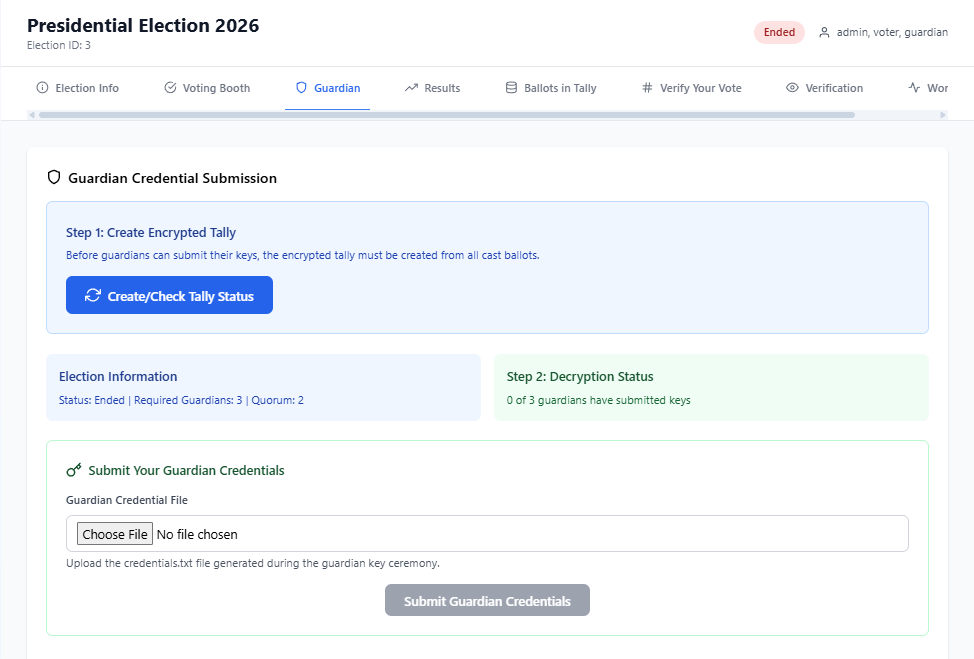
\includegraphics[width=\textwidth]{figures/afterElectionTallyCreation1.png}
		\caption{Tally creation in progress --- first stage}
		\label{fig:tally-creation-1}
	\end{subfigure}
	\hfill
	\begin{subfigure}[b]{0.48\textwidth}
		\centering
		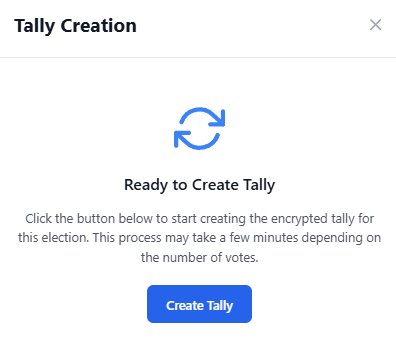
\includegraphics[width=\textwidth]{figures/afterElectionTallyCreation2.png}
		\caption{Tally creation in progress --- second stage}
		\label{fig:tally-creation-2}
	\end{subfigure}
	\caption{Tally creation progress stages}
	\label{fig:tally-creation-progress}
\end{figure}

\screenfig{afterElectionTallyCreatedSuccessfully.png}{Confirmation that the encrypted tally has been created successfully}

\begin{tcolorbox}[notebox]
	The tally computation is performed asynchronously in the background. For large elections (thousands of votes), this may take several minutes. You do not need to remain on the page --- progress is saved and you can return to check.
\end{tcolorbox}

% ────────────────────────────────────────────────────────────────────────────
\chapter{Cryptographic Decryption}
\label{ch:decryption}

This is the final cryptographic phase. The encrypted tally can only be decrypted by combining a minimum of \emph{quorum} guardian key shares.

\section{Partial Decryption (Guardian Action)}

\begin{enumerate}
	\item Guardians are notified that the tally phase is complete and partial decryption can begin.
	\item Each guardian navigates to the election page and opens the \uimenu{Guardian} tab.
	\item Click \uibutton{Upload Encrypted Key File} and select your private key file from Phase 1.

	      \screenfig{uploadCredentialFileForGuardianDecryption.png}{Uploading the encrypted private key file to begin partial decryption}

	\item Click \uibutton{Submit Credentials \& Decrypt}.

	      \screenfig{submitGuardianCredentialsToDecrypt.png}{Submitting guardian credentials to initiate partial decryption}

	\item The system will:
	      \begin{enumerate}
		      \item Decrypt your private key using your password (stored in database encrypted by ML KEM 1024).
		      \item Apply your private key to each tally chunk --- producing \textbf{partial decryptions} for your share.
		      \item Generate \textbf{compensated decryptions} for all other guardians (using the encrypted backup shares from Phase 2, decrypted with your private key). This allows the system to substitute for absent guardians.
		      \item Store all partial and compensated decryptions to the database.
	      \end{enumerate}
	\item A confirmation message is displayed when your decryption contribution is submitted.
\end{enumerate}

\begin{figure}[H]
	\centering
	\begin{subfigure}[b]{0.48\textwidth}
		\centering
		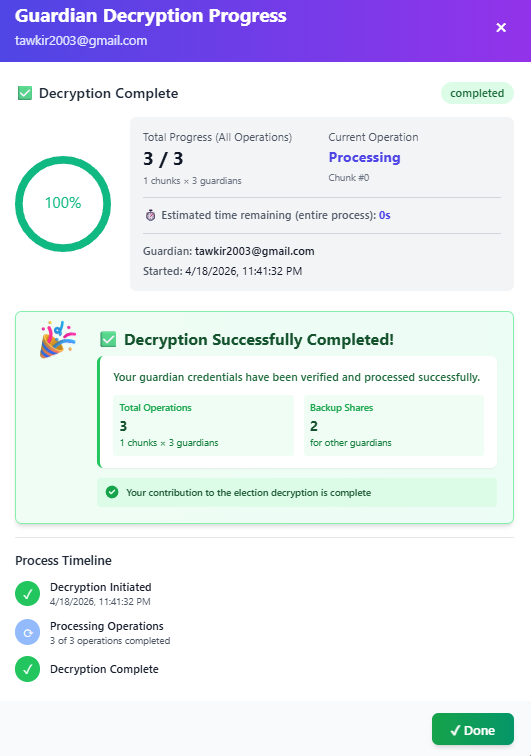
\includegraphics[width=\textwidth]{figures/successfulGuardianDecryption.png}
		\caption{Successful partial decryption submission}
		\label{fig:guardian-decrypt-success}
	\end{subfigure}
	\hfill
	\begin{subfigure}[b]{0.48\textwidth}
		\centering
		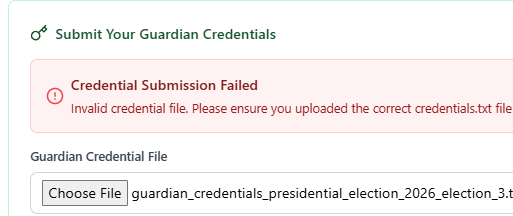
\includegraphics[width=\textwidth]{figures/wrongGuardianCredentialFile.png}
		\caption{Error: incorrect or mismatched credential file}
		\label{fig:guardian-decrypt-error}
	\end{subfigure}
	\caption{Guardian decryption outcomes: success (left) and credential error (right)}
	\label{fig:guardian-decrypt-outcomes}
\end{figure}

\screenfig{quorumNumberGuardiansDecrypted.png}{Dashboard showing quorum progress --- number of guardians who have submitted partial decryptions}

\begin{tcolorbox}[warnbox]
	The partial decryption process may take several minutes depending on the number of tally chunks. You can close the browser tab while decryption is running.
\end{tcolorbox}

\section{Combining Decryption Shares (Admin or Guardian)}

Once at least \emph{quorum} guardians have submitted their partial decryptions:

\begin{enumerate}
	\item Navigate to the election's \uimenu{Results} tab.
	\item The \uibutton{Combine Decryption Shares} button will become active.
	\item Click \uibutton{Combine Decryption Shares}.

	      \screenfig{combineDecryptionShares.png}{Combining decryption shares to produce the final plaintext tally}

	\item The system mathematically combines all submitted partial and compensated decryption shares to produce the \textbf{final plaintext tally}.
	\item The election results are now computed and published.
\end{enumerate}

\begin{tcolorbox}[tipbox]
	Results are displayed as a bar chart with vote counts per candidate, alongside percentage breakdowns and total ballot counts. All cryptographic proofs are also made available for public audit.
\end{tcolorbox}

\screenfig{electionResults.png}{Final election results page showing vote counts and candidate standings}

\begin{figure}[H]
	\centering
	\begin{subfigure}[b]{0.48\textwidth}
		\centering
		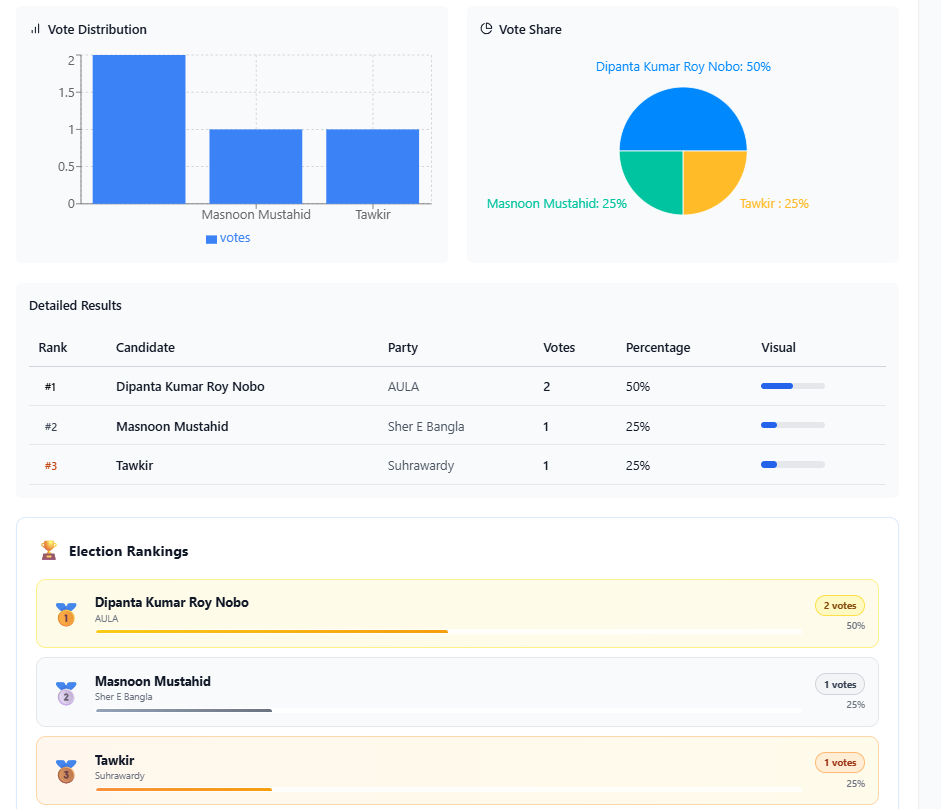
\includegraphics[width=\textwidth]{figures/electionResultsGraphsAndCharts.png}
		\caption{Election results displayed as graphs and charts}
		\label{fig:results-charts}
	\end{subfigure}
	\hfill
	\begin{subfigure}[b]{0.48\textwidth}
		\centering
		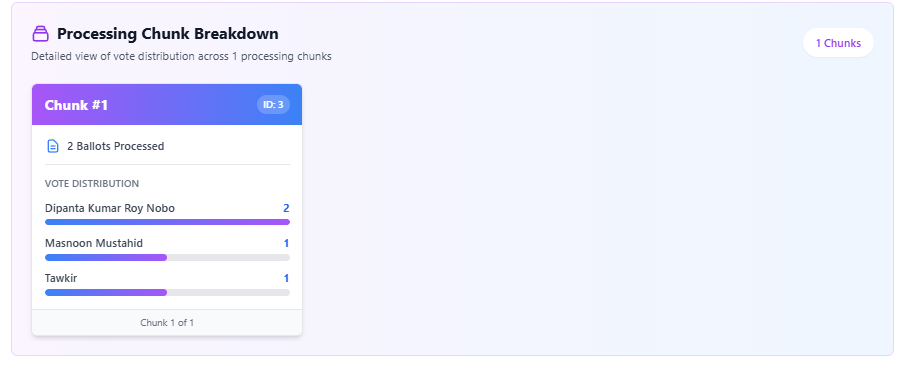
\includegraphics[width=\textwidth]{figures/electionResultsChunkBreakdown.png}
		\caption{Detailed chunk-level tally breakdown}
		\label{fig:results-chunks}
	\end{subfigure}
	\caption{Election results analytics: visual charts (left) and chunk tally breakdown (right)}
	\label{fig:results-analytics}
\end{figure}

% ════════════════════════════════════════════════════════════════════════════
\part{Verification \& Audit}

% ────────────────────────────────────────────────────────────────────────────
\chapter{Verifying Your Vote}
\label{ch:verification}

AmarVote is designed to be \textbf{fully auditable}. Every voter, every observer, and every independent researcher can verify the integrity of the election.

\section{Using Your Voter Receipt}

After the results are published:

\begin{enumerate}
	\item Navigate to the election page and open the \uimenu{Verify your vote} tab.



	\item Click \uimenu{Upload} and upload your ballot receipt you received in the email after your encrypted ballot was cast.

	      \screenfig{uploadYouBallotReceiptToVerify.png}{Uploading the ballot receipt file to initiate vote verification}

\end{enumerate}

The system will confirm:

\begin{itemize}
	\item \textbf{Ballot Found}: Your tracking code exists in the tally, confirming your ballot was \emph{recorded}.
	\item \textbf{Hash Match}: The ballot hash in the tally matches your receipt, confirming your ballot was \emph{not modified} after submission.
\end{itemize}

\screenfig{ballotVerifiedSuccessfully.png}{Successful ballot verification --- the system confirms the ballot was recorded and unmodified}

\begin{tcolorbox}[tipbox]
	If the ballot hash does not match, this indicates potential tampering. Report this immediately to the election administrator and your national or institutional election authority.
\end{tcolorbox}

\section{Manual Ballot Lookup}

If you prefer to verify without relying on the automated tool:

\begin{enumerate}
	\item Navigate to the election's \uimenu{Ballots in Tally} tab.
	\item This displays the complete list of all encrypted ballots included in the tally.

	      \screenfig{electionResultsballotsInTally.png}{The Ballots in Tally tab, listing all encrypted ballots included in the final tally}

	\item Manually search through the list for your Ballot Tracking Code.
	\item Compare the displayed ballot hash with the hash in your receipt email.
\end{enumerate}

\screenfig{seeIndividualEncryptedBallotContent.png}{Viewing the detailed content of an individual encrypted ballot in the tally}

\begin{tcolorbox}[notebox]
	This manual approach is deliberately available for maximum transparency. Ballot tracking codes are anonymised --- they identify the ballot but not the voter --- so this list is safe to make public.
\end{tcolorbox}

\section{Public Election Data Download}

All election data (except private keys) is publicly available for independent audit:

\begin{enumerate}
	\item Navigate to the election's \uimenu{Verification} tab.
	\item Click \uibutton{Download Election Data}.
	\item The download options:
	      \begin{itemize}
		      \item All encrypted ballots for chunks
		      \item Public keys of all guardians
		      \item The encrypted tally
		      \item All partial decryptions and proofs
		      \item The final plaintext results
	      \end{itemize}
\end{enumerate}
\screenfig{afterElectionVerificationTab.png}{The Verification tab on the election page, available after results are published}

\screenfig{downloadIndividualEncryptedBallots.png}{Downloading individual encrypted ballots for independent audit verification}

\begin{tcolorbox}[notebox]
	Any technically capable third party can use this downloaded data to re-verify the entire election independently using the ElectionGuard specification.
\end{tcolorbox}

% ════════════════════════════════════════════════════════════════════════════
\appendix

\chapter{Frequently Asked Questions}

\section*{Can the administrator see how I voted?}
No. Your ballot is encrypted using the combined public keys of all guardians before it is submitted. The administrator cannot decrypt individual ballots --- only the aggregate tally can be decrypted, and only with guardian cooperation.

\section*{What if a guardian is unavailable during decryption?}
If the number of available guardians meets or exceeds the quorum threshold, the election can still be tallied. The backup shares generated during Phase 2 are used to compensate for absent guardians.

\section*{Can I vote more than once?}
No. The system enforces a one-final-ballot-per-voter policy. While you can create and challenge multiple encrypted ballots (for verification purposes), casting your vote is a one-time action.

\section*{Is my identity linked to my ballot?}
Your voter receipt email contains a Ballot Tracking Code and Hash. Ballot hash mathematically derived from the \emph{encrypted} ballot --- they do not reveal your identity or your vote. The public tally list contains tracking codes but no voter names.
But for your privacy do not share the tracking code or ballot hash with anyone else, as they could be used to identify your encrypted ballot in the public tally. Though the ballot will still be encrypted, it is best practice to keep your receipt information private.

\section*{What is the Benaloh Challenge for?}
It is a cryptographic proof that the encryption software is working correctly --- that the encrypted ballot represents what you actually selected. It provides mathematical confidence without revealing your vote to the server.

\section*{What if I lose my guardian credentials?}
Immediately notify the election administrator. If the remaining guardians still meet the quorum threshold, tallying can proceed without you (using compensated decryption). If your loss would drop available guardians below quorum, the election results may be unrecoverable.

\chapter{Security Architecture Summary}

\begin{center}
	\begin{tabularx}{0.95\textwidth}{>{\bfseries}l X}
		\toprule
		\rowcolor{primaryblue}\color{white}Component & \color{white}Security Property                                              \\
		\midrule
		\rowcolor{lightgray}Ballot encryption        & ElectionGuard homomorphic encryption (El Gamal based)                       \\
		Private key storage                          & AES-256 encryption with guardian-chosen password                            \\
		\rowcolor{lightgray}Key distribution         & Shamir's Secret Sharing (threshold scheme)                                  \\
		Ballot verification                          & Zero-knowledge proofs included with each ballot                             \\
		\rowcolor{lightgray}Guardian backup          & Encrypted with each guardian's public key                                   \\
		Transit security                             & HTTPS/TLS (Nginx production configuration + Cloudflare Proxy Configuration) \\
		\rowcolor{lightgray}Authentication           & JWT tokens + optional TOTP 2FA                                              \\
		Password hashing                             & bcrypt (Spring Security default)                                            \\
		\rowcolor{lightgray}Infrastructure           & Docker containers, PostgreSQL, Redis, RabbitMQ                              \\
		\bottomrule
	\end{tabularx}
\end{center}

\end{document}